\subsubsection{Explicacion  QR}
Se plantea el nuevo sistema $Q^t A x = Q^t b$ que equivale a Rx = c, donde $\hat{c}$ son los primeros m elementos de c y d los restantes. El residuo s resulta s = c - Rx, donde los primeros m elementos de s son iguales a $\hat{c}$ - Rx y los restantes a d. De esta forma, el cuadrado del residuo, es decir, lo que se busca minimizar es igual a 

\begin{center}
$||$s$||^2_2$ = $||$ $\hat{c} - \hat{R}$x$||^2_2$ + $||$d$||^2_2$
\end{center}

Puesto que el segundo termino, d no depende de x, se busca minimizar el primero. Como $\hat{R}$ era no singular, entonces la solucion del sistema $\hat{R}$x = $\hat{c}$ es unica y es la solucion de cuadrados minimos. cabe destacar que el termino es la norma del residuo asociado con solucion obtenida.

\begin{figure}[H] 
\begin{center}
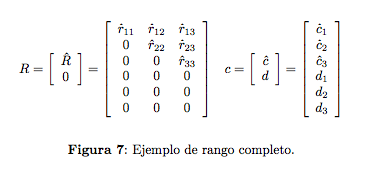
\includegraphics[width=0.6\textwidth]{img/exp-qr.png} 
\caption{Matriz de Givens} 
\end{center}
\end{figure}
